\chapter{Background on camera systems}
\label{ch:background}
Most real-time renderers use the simple pinhole camera model to create their images.
This approach leads to perfect images of the scene at a moment in time.
However to achieve a more realistic image or an artistic vision these images are to perfect, as they do not express real visual artefacts cameras and human eyes experience.
\section{Lens systems}
\label{ch:background-lens}
The simplest camera model is the pinhole camera.
An infinitesimal small hole is punched into an opaque material and creates the aperture.
An image is then taken from an image plane places at distance $d$ parallel to the aperture.
This camera model can be implemented easily in computer graphics software by modeling the aperture as a singe point in space.
The incoming light is then approximated by a ray emanating at an object or light source and crossing the aperture point.
This ray then intersects the image plane of the virtual camera at a single point and a color value is recorded.
This procedure is typically reversed for actual graphics pipelines with rays coming emanating at predetermined points on the image plane and crossing the aperture point.

If the aperture of a pinhole camera is assumed to be an infinitesimally small hole i.e. a point in space and light is approximated by straight rays, then the pinhole camera represents the ideal perspective camera.
Each point on the image plane only receives light from exactly one point and is therefore perfectly in focus.
The camera can therefore be described as a coordinate transformation $x_c, y_c, z_c \mapsto x, y$.
The resulting image coordinates $x, y$ can be derived from the equations:
\begin{align}
    \frac{x_c}{x} = -\frac{z_c}{d} \\
    \frac{y_c}{y} = -\frac{z_c}{d}
\end{align}
This results in the following projection:
\begin{align}
    \begin{pmatrix}
    x_c \\
    y_c \\
    z_c
\end{pmatrix} 
\mapsto
\begin{pmatrix}
    x \\
    y
\end{pmatrix}
= -\frac{d}{z_c}
\begin{pmatrix}
    x_c \\
    y_c
\end{pmatrix}
\end{align}
The negative sign represents the flipping of the image on the image plane \cite{Beyerer.2016}.

In reality this camera model suffers from multiple issues that make pinhole cameras unpractical for photography.
The most obvious problem is the impossibility to create a infinitesimally small hole.
As such the hole will always have a real diameter $D$.
This causes a point on the image plane to receive light from multiple sources and thus negates the theoretically perfect focus of the pinhole camera.
If one still tries to approach a $D$ of $0$ the light entering the pinhole will also approach $0$.
The image will become darker or the exposure time needed for a bright image will approach infinity.
Additionally at such small values of $D$ the assumption of light as a ray will break down and one will notice diffraction start to appear and blurring the image further \cite{Beyerer.2016}.

\begin{figure}[h]
    \centering
    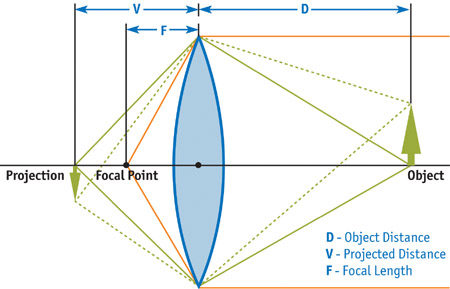
\includegraphics[width=0.8\textwidth]{images/fig23-01_1.png}
    \caption{Optical mapping of a thin-lens}
    \label{fig:thin-lens}
    \cite{Demers.2005}
\end{figure}

To increase the amount of light hitting the image plane one or more lenses are used in real camera systems.
In the following we will only describe single thin-lens system, as they are sufficient to demonstrate the most important visual phenomena.
Lenses are used to bundle all light entering parallel to the optical axis at the focal point of the lens.
The relation between the radius of the lens $R$ and the distance of the focal point $F$ to the lens can be described as
\begin{align}
    R = 2 F \frac{n_2 - n_1}{n_1}
\end{align}
with $n_1$ representing the refractive index of the surrounding material and $n_2$ the refractive index of the lens \cite{Beyerer.2016}.

Most lens system are constructed with rotational symmetry with the light entering at small angles $\alpha$ between the light ray and the optical axis.
As such the approximation $\sin  \alpha \approx \alpha$ holds and we can linearize the law of refraction to
\begin{align}
    n_1 \sin \theta_1 = n_2 \sin \theta_2 \rightarrow n_1 \theta_1 = n_2 \theta_2.
\end{align}
This approximation is called paraxial approximation and enables the modeling of spherical lenses as linear systems with their associated matrices. \cite{Beyerer.2016}

The relation between the object and image can be described with
\begin{align}
    \frac{1}{F} &= \frac{1}{D} + \frac{1}{V} \\
    \frac{Size\:of\:object}{F} &= -\frac{Size\:of\:image}{V-F}.
    \label{eq:sharp-thin-lens}
\end{align}

As such the \gls{dof} of a camera with a distance is limited to a single plane with distance $P$.

\begin{figure}[h]
    \centering
    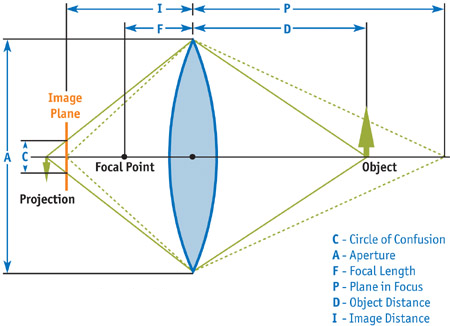
\includegraphics[width=0.8\textwidth]{images/fig23-02_1.png}
    \caption{Thin lens with imperfect focus}
    \label{fig:coc-thin-lens}
    \cite{Demers.2005}
\end{figure}
However a perfectly sharp image is not necessary as an image sensor cannot resolve details smaller than a certain size.
This lower limit is typically given by the physical size of the sensor pixels.
We therefore have a range of values of $D$ such that the image still appears in focus.
Using similar triangles we can derive the equation
\begin{align}
    \frac{C}{A} = \frac{D-I}{D} \implies C = A \cdot |\frac{D-I}{D}|.
    \label{eq:coc}
\end{align}
To have more control over the camera, the equation can be expanded to:
\begin{align}
    C = | A \cdot \frac{F(P-D)}{D(P-F)}|.
    \label{eq:coc-expanded}
\end{align}
$C$ describes the radius of the image a single dot on the image plane and is called \gls{coc}.
This equation can be used to derive the following equation for \gls{dof}:
\begin{align}
    |P-D| = |P-D|(A) = \frac{C \cdot D}{\frac{A F}{P-F} - C}
    \label{eq:dof}
\end{align}
A few notes on equation \ref{eq:coc} and \ref{eq:dof}:
\begin{itemize}
    \item Pinhole cameras have a diameter $A$ of 0 and thus perfect focus. Any real lens, including the human eye has a $A$ greater than 0.
    \item To increase the \gls{dof} $A$ is typically reduced by the use of an aperture at the expense of image brightness.
    \item The \gls{coc} increases much faster in the foreground than in the background.
\end{itemize}

The blur of optical system can be described by its \gls{psf}.
It characterizes the spread of a single point source of light onto the image plane and takes into account the many factors that contribute to a blurring of the image.
This includes, but is not limited to, imperfections in the lens, the shape of the aperture, diffraction effects and spherical and chromatic aberrations.
The \gls{psf} is typically represented as a two-dimensional function with a Gaussian or disk-like shape.
When thinking of an optical system as a function $f$ that transform incoming light rays into an image, the \gls{psf} represents its impulse response function \cite{Beyerer.2016}.
The ability to define the particular \gls{psf} used is important to simulate particular camera systems accurately.

\begin{figure}
    \centering
    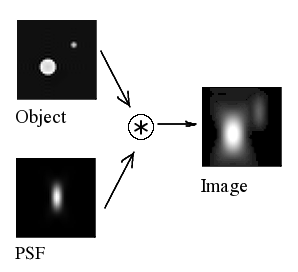
\includegraphics[width=0.6\textwidth]{images/Convolution_Illustrated_eng.png}
    \caption{Light source convoluted with \gls{psf} \cite{psf}}
    \label{fig:psf}
\end{figure}

\section{Sensor}
In contrast to a virtual camera an image sensor cannot interrogate the color of an object, but must wait for light to hit its light sensors and produce a strong enough image.
During the capture of a frame the view of a point camera can be described by
\begin{align}
    I(\omega) = \int_{\Delta T} f(\omega,t) L(\omega,t)dt.
    \label{eq:mb-integral}
\end{align}
Where $\omega$ is the direction of the incoming light, $L(\omega,t)$ is the incoming radiance and $f(\omega,t)$ models the influence of the optical system.
This equation can be adjusted to be more applicable to computer-graphics systems as
\begin{align}
    I_{xy} = \sum_l \int_\Omega \int_{\Delta T} f(\omega, t) g_l(\omega, t) L_l(\omega, t) \: dt \: d\omega.
    \label{eq:mb-cg-integral}
\end{align}
Here the pair $(x,y)$ represent the coordinates of the image pixel.
The geometry of each object is accounted for by iterating over all objects $l$.
To also account for the occlusion of objects in the scene $g_l(\omega, t)$ that is 1 if the object $l$ is directly visible and 0 if not.
Even though $g_l(\omega, t)$ does not account for transparent or reflective objects, this is not a limitation of the model as the term $L_l(\omega, t)$ accounts for these situations.
$L_l(\omega, t)$ simply describes what light is coming from angle $\Omega$ at time $t$ without describing the method how this is achieved. \cite{Navarro.2011}
For any computer-generated images the renderer must approximate this integral.

The effects of motion blur are often unwanted, especially in photography, and are reduced with lowering the exposure time of the image sensor.
This leaves less time for light to enter the sensor and therefore reduces image brightness.
To compensate for this either the sensitivity of the sensor (ISO) must be increased or the aperture must be widened to increase the amount of light entering.
Both options come with trade-offs to image quality.
Increasing the sensor sensitivity also introduces noise to the final image, while increasing the aperture diameter reduces the \gls{dof} (see equation \ref{eq:dof}).

% only digital image sensors considered
% sensors are exposed for a fixed length of time for each image
% longer time increases brightness but causes blurring of moving objects
% low brightness can be compensated with higher iso at cost of higher noise
% sensors can be exposed all at once or one line at a time
% bright light spills over into neighbouring pixels (bloom)
% pixels are layed out in special patterns  (beyer)
% the color of a pixel in a frame can be described as an integral over all angels over the exposure time